\chapter{진동자, 점유수, 그리고 최초의 양자장}

양자장론은 중력을 제외하고 알려진 거의 모든 물리 현상을 다루는 틀이다. 그렇다고 모든 문제를 풀 수 있다는 뜻은 아니다. 수소 원자는 다룰 만하지만, 붕소 같은 원자에 이르면 계산은 벌써 훨씬 어려워지고, 사람은 현실적으로 어떤 장론 계산으로도 다룰 수 없을 만큼 복잡하다. 이 틀은 근본적일 수 있지만, 그 방정식은 여전히 감당하기 어려울 만큼 풀기 힘들 수 있다.

그러므로 가능한 한 가장 기초적인 방식으로 시작하겠다. 이 주제는 때때로 \emph{제2양자화}라고 불리지만, 필요한 수학적 장치를 갖추기 전까지는 그 이름만으로 알 수 있는 것이 거의 없다. 가장 짧은 길은 상대론적 장이 아니라 조화진동자에서 출발하는 것이다. 용수철 자체가 핵심은 아니다. 중요한 것은 생성 연산자와 소멸 연산자의 대수다. 이 대수를 여러 모드에 반복 적용하면, 생성 연산자는 더는 단지 ``진동자를 한 에너지 준위 올리는 것''을 뜻하지 않고 문자 그대로 ``입자를 생성하는 것.''을 뜻하게 된다.

\section{대수로서의 진동자}

진동자 하나에 대해 \(a^\dagger\)를 들뜸을 높이는 연산자로, \(a\)를 낮추는 연산자로 두자. 표기 \(a_+\)와 \(a_-\)도 같은 뜻이지만, 대거 표기는 장론에서 쓰는 표현을 미리 보여 준다. 바닥 상태는 다음을 만족한다.
\begin{equation}
a|0\rangle=0,
\end{equation}
수 연산자는 다음과 같다.
\begin{equation}
N=a^\dagger a,
\qquad
N|n\rangle=n|n\rangle.
\end{equation}
두 사다리 연산자는 서로 에르미트 수반이며, 핵심 교환자는 다음과 같다.
\begin{equation}
[a,a^\dagger]=1.
\label{eq:l06-single-commutator}
\end{equation}
이 간단한 대수가 진동자의 거의 전부다.

위치와 운동량의 적절한 선형결합으로 \(a\)와 \(a^\dagger\)를 복원할 수 있다. 정확한 규약은 \(x\), \(p\), \(m\), \(\omega\)의 정규화에 따라 달라진다. 여기서 유용한 불변적 진술은 \(a^\dagger a\)가 바닥 상태 에너지에 해당하는 가산 상수항을 제외한 조화 진동자의 이차 해밀토니안을 재구성한다는 것이다. 따라서
\begin{equation}
H=\hbar\omega\left(N+\frac12\right).
\end{equation}
지금 논의에서는 상수항을 버리고 다음과 같이 다룬다.
\begin{equation}
H=\hbar\omega N.
\label{eq:l06-one-oscillator-hamiltonian}
\end{equation}
진동수는 한 번 들뜨는 데 필요한 에너지를 알려 준다. \(n\)을 하나 높이는 데 \(\hbar\omega\)의 에너지가 들고, \(n\)을 하나 낮추면 같은 양의 에너지가 방출된다.

\section{서로 독립인 여러 진동자}

이제 진동자를 여러 개 두고 \(i\)로 번호를 붙이자. 이 표기는 지표일 뿐, 허수 단위가 아니다. 모드의 수는 유한할 수도 무한할 수도 있다. 여러 개의 독립된 용수철이 한 가지 그림을 제공하고, 이상적인 바이올린 현의 정상 모드가 또 다른 그림을 제공한다. 장론 응용에서는 무한히 많은 모드가 중요하다.

독립성에는 연산자적 의미가 있다. 실제로 독립된 부분계에 속한 연산자는 서로 교환한다. 그렇지 않다면 해당 물리량들을 독립적으로 측정할 수 없고, 애초에 계들이 독립적이지도 않을 것이다. 따라서 다음이 성립한다.
\begin{align}
[a_i,a_j]&=0, \\
[a_i^\dagger,a_j^\dagger]&=0, \\
[a_i,a_j^\dagger]&=\delta_{ij}.
\label{eq:l06-many-commutators}
\end{align}
\(i\ne j\)이면 두 모드에 속하는 모든 연산자가 서로 교환한다. \(i=j\)이면 마지막 줄은 식~\eqref{eq:l06-single-commutator}으로 줄어든다.

각 진동자는 고유한 수 연산자와, 일반적으로 고유한 진동수를 갖는다.
\begin{equation}
N_i=a_i^\dagger a_i,
\qquad
H=\sum_i\hbar\omega_i N_i.
\label{eq:l06-many-hamiltonian}
\end{equation}
동시 고유상태에는 다음 전체 목록을 붙여 이름을 정한다.
\begin{equation}
|n_1,n_2,n_3,\ldots\rangle,
\qquad n_i=0,1,2,\ldots.
\label{eq:l06-occupation-ket}
\end{equation}
정수 \(n_i\)는 \(i\)번째 진동자의 \emph{점유수}라고 한다. 지금은 그저 용어일 뿐이다. 곧 이것은 한 입자 상태를 점유한 입자 수를 세게 되며, 이 이름은 문자 그대로의 뜻을 갖게 된다.

모든 점유수가 0인 상태는 다음과 같다.
\begin{equation}
|0\rangle\equiv|0,0,0,\ldots\rangle,
\qquad a_i|0\rangle=0\quad\text{for every }i.
\label{eq:l06-oscillator-vacuum}
\end{equation}

\begin{classroomqa}\lecturetimestamp{00:15:27}\audiencequestion{진동자가 무한히 많으면 바이올린 현 같은 계의 연속적인 모드에 해당하나요?}\lecturerresponse{이상화된 현에서는 그렇습니다. 실제 현은 원자로 이루어져 있으므로, 파장이 충분히 짧아지면 결국 미시적인 차단 규모에 이릅니다. 그래도 연속체 모형은 장론에서 쓰이는 무한한 모드 집합의 동기가 됩니다.}\end{classroomqa}

\section{사다리 계수가 제곱근인 이유}

\(a^\dagger\)는 \(N\)의 고유상태를 다음 고유상태로 올려야 하지만, 정규화만으로 계수가 정해지지는 않는다.
\begin{equation}
a^\dagger|n\rangle=c_n|n+1\rangle.
\label{eq:l06-unknown-coefficient}
\end{equation}

\begin{figure}[htbp]\centering
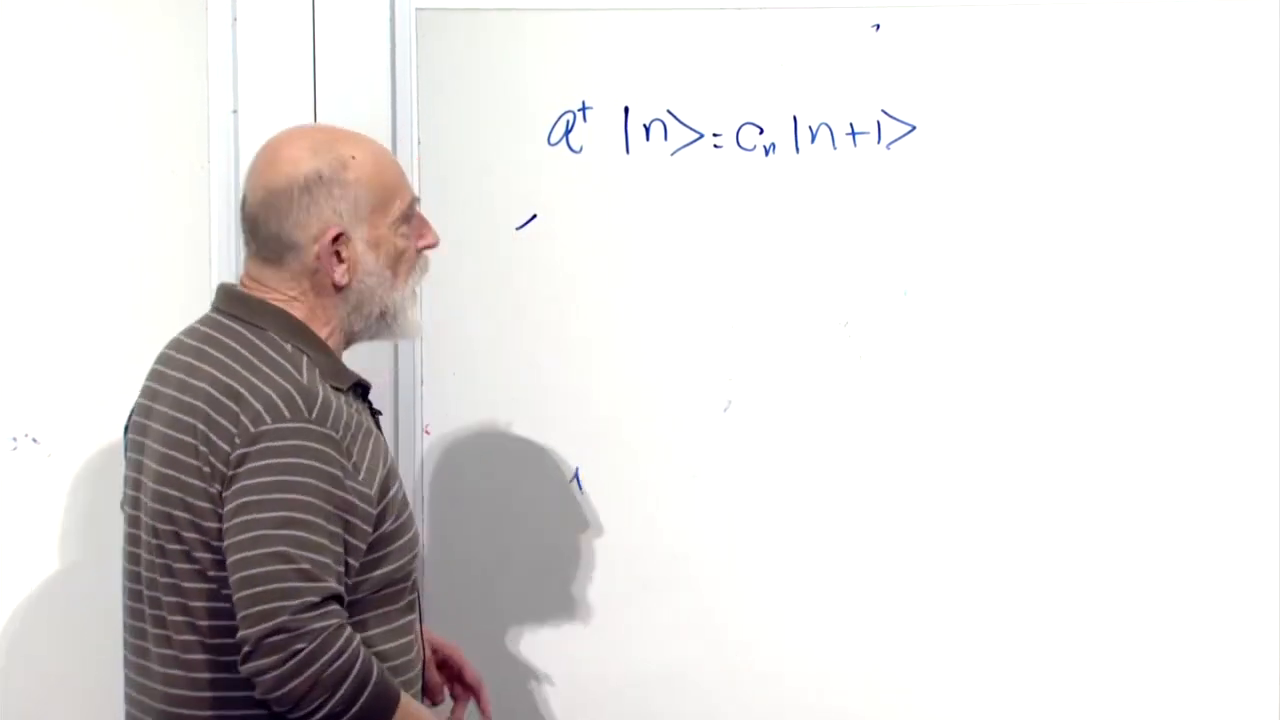
\includegraphics[width=0.9\linewidth]{lecture_06_frame_01.png}\caption{사다리 계수는 정규화를 유도하기 전에 먼저 도입한다. 판서의 방정식은 식~\eqref{eq:l06-unknown-coefficient}에 재현했다.}\lectureframe{00:19:38}\end{figure}

\(c_n\)가 실수가 되도록 위상 규약을 택하자. 에르미트 수반을 취하면 다음을 얻는다.
\begin{equation}
\langle n|a=c_n\langle n+1|.
\end{equation}
두 관계식을 곱하고 정규화된 기저 상태를 사용하면,
\begin{align}
c_n^2
&=\langle n|aa^\dagger|n\rangle \\
&=\langle n|(a^\dagger a+1)|n\rangle \\
&=\langle n|(N+1)|n\rangle \\
&=n+1.
\end{align}
따라서
\begin{equation}
a^\dagger|n\rangle=\sqrt{n+1}\,|n+1\rangle.
\label{eq:l06-raising-rule}
\end{equation}

\begin{classroomqa}\lecturetimestamp{00:22:35}\audiencequestion{\(\langle n+1|n+1\rangle=1\)로 놓고 나서 \(c_n\)를 구해도 되는 이유는 무엇인가요?}\lecturerresponse{고유벡터는 처음부터 정규화된 기저로 택한다. 이들의 정규화가 \(a^\dagger|n\rangle\)의 정규화를 정해 주지는 않는다. 남아 있는 바로 그 정보가 계수 \(c_n\)다.}\end{classroomqa}

낮춤 규칙도 같은 방식으로 얻어진다.
\begin{equation}
a|n\rangle=\sqrt n\,|n-1\rangle.
\label{eq:l06-lowering-rule}
\end{equation}
\(n=0\)에서는 계수가 자동으로 0이 되므로, 이 규칙에는 \(a|0\rangle=0\)도 포함된다. 모드가 여러 개일 때 연산자는 자기 모드의 점유수만 바꾼다.
\begin{align}
a_i^\dagger|n_1,\ldots,n_i,\ldots\rangle
&=\sqrt{n_i+1}\,|n_1,\ldots,n_i+1,\ldots\rangle, \\
a_i|n_1,\ldots,n_i,\ldots\rangle
&=\sqrt{n_i}\,|n_1,\ldots,n_i-1,\ldots\rangle.
\label{eq:l06-multimode-ladders}
\end{align}
다른 성분에는 아무 변화도 없다.

\section{파동함수는 양자장이 아니다}

장을 정의하기 전에 익숙한 파동함수와 구별해야 한다. 세 가지 차이가 이 전환을 정리해 준다.

첫째, 한 입자 파동함수
\begin{equation}
\psi(x)=\langle x|\psi\rangle
\end{equation}
는 상태벡터의 표현이다. 파동함수 자체가 관측량인 것은 아니다. 우리는 위치, 운동량, 각운동량 및 다른 연산자들을 측정한다. 파동함수는 그 측정 결과의 확률을 계산하는 데 필요한 진폭을 제공한다.

둘째, 다입자 파동함수는 모든 입자의 위치에 의존한다. 위치벡터를 잠시 \(x\)와 \(y\)라고 부르는 두 입자의 경우,
\begin{equation}
\psi(x,y)=\langle x,y|\psi\rangle.
\end{equation}
여기서 \(x\)와 \(y\)는 서로 다른 두 입자를 나타낸다. 하나의 위치벡터의 데카르트 \(x\) 성분과 \(y\) 성분이 아니다. \(N\)개의 입자에 대해서는 상태를 다음과 같이 나타낸다.
\begin{equation}
\psi(x_1,x_2,\ldots,x_N).
\end{equation}

셋째, 이 파동함수는 고정된 입자 수를 기술한다. 입자가 15개인 파동함수에는 위치 인자가 15개 있고, 15입자 힐베르트 공간에 속한다. 이것만으로는 입자 수가 15개에서 14개나 16개로 바뀌는 과정을 기술하지 못한다.

양자장은 이 특징들을 뒤집는다. 아래에서 도입할 장은 상태가 아니라 연산자이고, 공간의 한 점 \(x\)에 의존하며, 입자 수가 다른 모든 부문을 포함하는 상태공간에 작용한다. ``한 점''이라는 말은 자유롭게 변할 수 있는 위치벡터 하나를 뜻한다. \(x\)에 하나의 수치값을 지정했다는 뜻은 아니다.

나중에 중요해질 단서가 하나 있다. 아래에서 도입할 장 \(\Psi(x)\)는 에르미트가 아니므로 엄밀한 의미에서 그 자체가 관측량은 아니다. 그 에르미트 결합이 관측량이다. 따라서 장을 측정할 수 있다는 잠정적 진술은 폐기되는 것이 아니라 더 정확해진다. 장은 연산자값 함수이고, 그 에르미트 결합이 측정 가능한 물리량을 나타낸다.

\begin{classroomqa}\lecturetimestamp{00:36:52}\audiencequestion{장이 한 위치의 함수라면 그 위치는 변할 수 있나요? 그리고 두 입자 파동함수에서 \(y\)는 어떻게 된 건가요?}\lecturerresponse{점 \(x\)는 공간 전체를 두루 변한다. ``한 위치''란 연산자에 공간 인자가 하나 있다는 뜻이지, 그 인자가 고정되어 있다는 뜻은 아니다. \(\psi(x,y)\)에서 기호 \(x\)와 \(y\)는 두 입자의 위치를 나타내며, 같은 뜻으로 \(x_1\)와 \(x_2\)라고 쓸 수 있다. 이들은 장의 인자를 이루는 두 데카르트 성분이 아니다.}\end{classroomqa}

\begin{classroomqa}\lecturetimestamp{00:38:15}\audiencequestion{고정된 입자 수를 쓰는 파동함수 기술과 장 기술은 어떻게 연결되나요? 서로 다른 종류의 입자를 기술하나요?}\lecturerresponse{그 연결은 앞으로 살펴볼 핵심 구성이다. 입자들은 같은 종류다. 이번 강의에서는 보손을 다룬다. 페르미온에는 다른 대수가 필요하다.}\end{classroomqa}

\section{상자 속 한 입자}

잠시 보통의 한 입자 양자역학으로 돌아가자. 입자를 일차원 상자에 넣는다. 입자가 하나뿐이면 보손과 페르미온의 구별은 중요하지 않다. 교환이나 배타성을 따져 볼 두 번째 동일 입자가 없기 때문이다.

에너지 고유함수를
\begin{equation}
\psi_1(x),\ \psi_2(x),\ \psi_3(x),\ldots
\end{equation}
라고 하자. 가장 낮은 모드는 벽에서 0이 되는 가장 매끄러운 파동이다. 다음 모드에는 내부 마디가 하나 있고, 에너지가 높아질수록 모드는 더 빠르게 진동한다. 폭이 \(L\)인 이상적인 무한 사각 우물에서는 다음과 같이 정규화된 기저를 편리하게 쓸 수 있다.
\begin{equation}
\psi_i(x)=\sqrt{\frac{2}{L}}\sin\!\left(\frac{i\pi x}{L}\right),
\qquad 0<x<L.
\label{eq:l06-box-basis}
\end{equation}
명시적인 사인 함수 식은 칠판에 그린 정성적 스케치를 표준적인 형태로 구현한 것이다. 아래 논증에는 완비 정규직교 집합을 이루는 단일 입자 상태들만 있으면 된다.

\begin{figure}[htbp]\centering
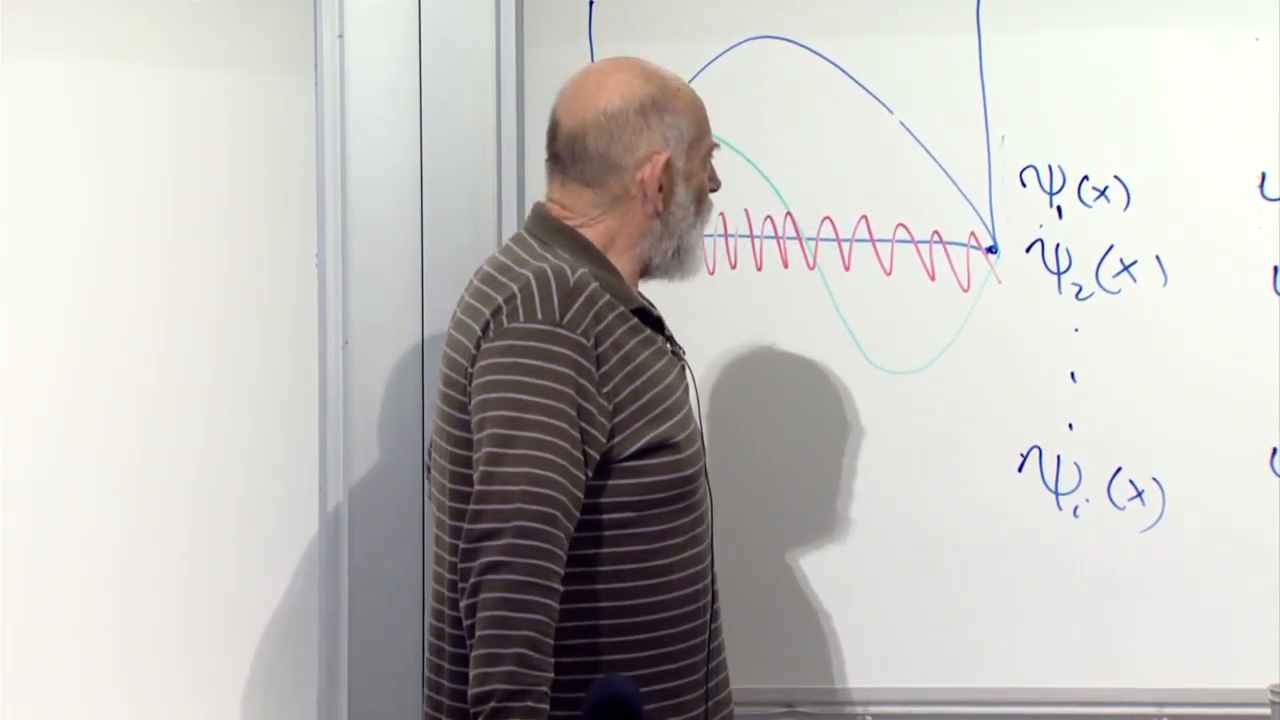
\includegraphics[width=0.9\linewidth]{lecture_06_frame_03.png}\caption{에너지가 낮은 순으로 배열한 상자 속 한 입자 모드. 첫 번째 모드에는 내부 마디가 없고, 두 번째 모드에는 하나 있으며, 생략한 더 높은 모드일수록 점점 더 빠르게 진동한다.}\lectureframe{00:43:10}\end{figure}

실시간 판서의 가림을 피해서 같은 구조를 다시 그리면 다음과 같다.
\begin{figure}[htbp]\centering
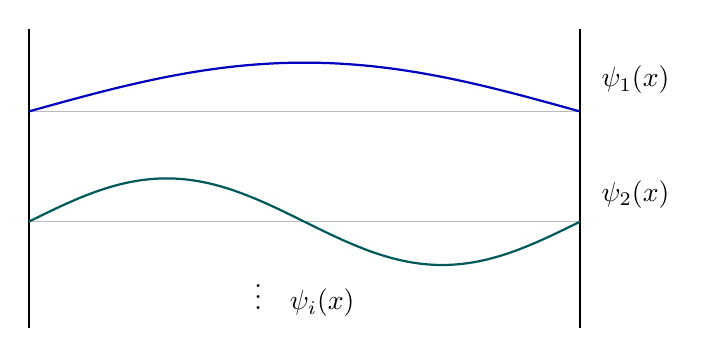
\begin{tikzpicture}[x=1cm,y=1cm]
  \draw[thick] (0,0) -- (0,3.8);
  \draw[thick] (7,0) -- (7,3.8);
  \draw[gray!55] (0,2.75) -- (7,2.75);
  \draw[gray!55] (0,1.35) -- (7,1.35);
  \draw[blue!75!black,thick,domain=0:7,samples=120]
    plot (\x,{2.75+0.62*sin(180*\x/7)});
  \draw[teal!70!black,thick,domain=0:7,samples=120]
    plot (\x,{1.35+0.55*sin(360*\x/7)});
  \node[right] at (7.15,3.15) {$\psi_1(x)$};
  \node[right] at (7.15,1.70) {$\psi_2(x)$};
  \node at (3.5,0.45) {$\vdots\quad \psi_i(x)$};
\end{tikzpicture}\caption{정성적인 상자 모드 그림을 깔끔하게 재구성했다. 고유함수들을 알아보기 쉽게 세로 방향으로 떨어뜨려 그렸으며, 이 간격은 추가적인 물리 좌표가 아니다.}\end{figure}

지표 \(i\)는 한 입자 상태를 나타내며, 입자나 마디의 수를 나타내지 않는다. 상자 기저에서는 \(i\)가 내부 마디 수보다 하나 큰 값인 것이 우연히 성립한다. 각 상태는 에너지 \(\varepsilon_i\)를 갖는다. 강의 표기를 따라 이 에너지를 \(\hbar\omega_i\)라고 쓸 수도 있고, \(\hbar=1\)로 놓은 뒤에는 간단히 \(\omega_i\)라고 쓸 수도 있다.

\begin{classroomqa}\lecturetimestamp{00:39:01}\audiencequestion{앞서 가정한 독립성은 정확한가요? 그리고 지표 \(i\)를 원자 속 전자의 가능한 상태에 붙일 수도 있나요?}\lecturerresponse{독립 모드 구성에서는 서로 다른 모드 사이의 교환 관계가 정확히 성립한다. 이 지표를 한 입자 원자 상태에 붙일 수도 있다. 하지만 입자들이 상호작용하면 간단한 독립 모드 해밀토니안만으로는 전체를 설명할 수 없다.}\end{classroomqa}

\begin{classroomqa}\lecturetimestamp{00:40:34}\audiencequestion{상자 속 입자는 보손인가요?}\lecturerresponse{보손일 수도 있지만, 입자가 하나뿐이면 통계는 중요하지 않다. 배타성과 교환은 동일한 입자가 둘 이상일 때에만 의미가 있다.}\end{classroomqa}

\section{상자 모드에서 포크 공간으로}

이제 상자 안에 동일한 보손을 원하는 수만큼 허용하자. 어떤 수 \(n_1\)의 입자가 \(\psi_1\)에 있을 수 있고, 어떤 수 \(n_2\)의 입자가 \(\psi_2\)에 있을 수 있으며, 이런 식으로 이어진다. 따라서 기저 상태는 다음과 같다.
\begin{equation}
|n_1,n_2,n_3,\ldots\rangle.
\end{equation}
이는 여러 진동자에 대해 이미 사용한 표기와 정확히 같다. 이 대응은 구조적인 것이다. 한 입자 상태마다 진동자 하나를 대응시키고, 그 진동자의 들뜸 수를 해당 상태를 점유한 입자 수와 동일시한다.

여기서는 보손이라는 점이 핵심이다. 보손의 경우 각 \(n_i\)는 음이 아닌 정수라면 어떤 값이든 될 수 있다. 페르미온의 경우 한 입자 상태는 비어 있거나 하나의 입자만 점유할 수 있고, 두 입자 이상이 점유할 수는 없다. 따라서 보통의 진동자 대수를 그대로 사용할 수 없다.

이제 점유수 기저에 대한 작용으로 연산자를 정의할 수 있다. 연산자 \(a_i^\dagger\)는 한 입자 상태 \(i\)에 입자 하나를 생성하고, \(a_i\)는 하나를 소멸시킨다.
\begin{align}
a_i^\dagger|n_1,\ldots,n_i,\ldots\rangle
&=\sqrt{n_i+1}\,|n_1,\ldots,n_i+1,\ldots\rangle, \\
a_i|n_1,\ldots,n_i,\ldots\rangle
&=\sqrt{n_i}\,|n_1,\ldots,n_i-1,\ldots\rangle.
\end{align}
이것은 사후에 붙인 비유가 아니다. 이 기저에서 보손 생성 연산자와 소멸 연산자를 정의하는 방식이다. 기저가 공간 전체를 생성하므로 이 정의는 선형성에 따라 모든 상태에 대한 연산자의 작용을 정한다.

\begin{classroomqa}\lecturetimestamp{00:47:11}\audiencequestion{\(n_1,n_2,n_3\)가 양자 상태인가요?}\lecturerresponse{표지 \(1,2,3,\ldots\)은 한 입자 상태를 가리킨다. 기호 \(n_1,n_2,n_3,\ldots\)는 그 상태들을 점유한 입자 수다. 상태 표지와 그 점유수를 구별하는 것이 표기에서 가장 주의할 점이다.}\end{classroomqa}

\subsection{제곱근 인자의 역할}

인자 \(\sqrt{n_i+1}\)는 입자를 하나 더 나타내거나 별도의 물리 과정에 해당하지 않는다. 연산자가 올바른 정규화와 대수를 갖도록 하는 인자다. 한 모드에서,
\begin{align}
a a^\dagger|n\rangle
&=a\bigl(\sqrt{n+1}\,|n+1\rangle\bigr) \\
&=(n+1)|n\rangle,
\end{align}
한편,
\begin{equation}
a^\dagger a|n\rangle=n|n\rangle.
\end{equation}
그러므로 두 결과의 차이는 \(|n\rangle\)이며, 이는 \([a,a^\dagger]=1\)에 필요한 결과다. 두 사다리 연산자는 대략 각각 \(\sqrt n\) 정도의 크기를 갖는다. 두 연산자의 곱이 대략 \(n\) 크기의 수 연산자를 주기 때문이다.

\begin{classroomqa}\lecturetimestamp{00:47:52}\audiencequestion{제곱근 인자는 구체적으로 어떤 물리적 의미를 갖나요?}\lecturerresponse{주로 수학적인 정규화 인자다. 점유 상태가 정규화되도록 하고, \(a^\dagger a\)의 고유값이 \(n\)가 되도록 하며, 사다리 연산자들이 진동자 교환자를 만족하도록 한다. 때로는 필요한 의미가 수학 그 자체다.}\end{classroomqa}

\begin{classroomqa}\lecturetimestamp{00:52:25}\audiencequestion{생성 연산자와 소멸 연산자는 성질과 기저에 대한 작용으로만 정의했나요?}\lecturerresponse{그렇다. 정의가 더 근본적인 그림에서 나와야 하는 것은 아니다. 정의의 가치는 그 결과로 판단한다. 완비 기저에 대한 작용을 정의하면 연산자가 모든 곳에서 정의되고, 이 정의들은 원하는 교환 관계를 재현한다.}\end{classroomqa}

\begin{classroomqa}\lecturetimestamp{00:53:22}\audiencequestion{왜 \(a_i\)는 입자를 다른 상태로 옮기기만 하는 것이 아니라 사라지게 하나요?}\lecturerresponse{\(a_i\)는 상태 \(i\)의 점유수를 낮추도록 정의되기 때문이다. 유용한 질문은 정의가 왜 참인지가 아니라 왜 유용한지다. 방출과 흡수에는 입자 수를 바꾸는 연산자가 필요하므로 이 정의가 유용하다. 복사가 방출될 때 광자가 생성되고 흡수될 때 소멸한다.}\end{classroomqa}

모든 점유수 상태가 생성하는 공간을 \emph{포크 공간}이라 한다. 이 공간에는 진공, 모든 한 입자 상태, 모든 두 입자 상태 등이 고정된 상한 없이 들어 있다.
\begin{equation}
\mathcal F=\mathcal H_0\oplus\mathcal H_1\oplus\mathcal H_2\oplus\cdots.
\label{eq:l06-fock-space}
\end{equation}
직합 표기는 보통의 \(N\)입자 파동함수로는 드러나지 않던 사실, 즉 모든 입자 수 부문이 하나의 상태공간에 속한다는 점을 분명히 보여 준다.

\begin{classroomqa}\lecturetimestamp{00:54:56}\audiencequestion{점유수 고유벡터에 연산자를 정의하면 임의의 벡터에 대한 작용도 정해지나요? 그러면 진동자 교환 관계가 따라오나요?}\lecturerresponse{정확하다. 점유수 벡터들이 기저를 이루므로 선형성에 따라 정의가 포크 공간 전체로 확장된다. 그 기저에 연산자를 작용시키면 보손 교환 관계가 성립함을 확인할 수 있다. 한 입자 상태마다 진동자 하나를 대응시키며, 그 상태에서 진동자의 점유수는 그 상태에 있는 입자 수다.}\end{classroomqa}

\subsection{진공과 자유 해밀토니안}

포크 진공은 어떤 한 입자 상태도 점유되지 않은 상태다.
\begin{equation}
|0\rangle=|0,0,0,\ldots\rangle,
\qquad a_i|0\rangle=0.
\end{equation}
여기서 \emph{바닥 상태}라는 말은 오해를 부를 수 있다. 가장 낮은 \emph{한 입자} 상태는 모드 \(i=1\)다. 포크 진공에서는 그 모드에도 입자가 없다. 입자가 최저 모드에 있다면 \(a_1\)가 그 입자를 제거해 계를 진공으로 되돌릴 수 있다.

\begin{classroomqa}\lecturetimestamp{00:56:19}\audiencequestion{점유수 표기에서 진공은 무엇인가요? 최저 한 입자 상태가 점유되어 있나요?}\lecturerresponse{진공에서는 모든 점유수가 0이고 모든 \(a_i\)가 진공을 소멸시킨다. 최저 한 입자 모드는 진공에서 점유되지 않는다. 점유되어 있다면 그 모드의 소멸 연산자가 해당 입자를 제거할 수 있다.}\end{classroomqa}

비상호작용 입자의 전체 에너지는 각 입자의 에너지를 더한 값이다. 상태 \(i\)에 있는 입자 하나의 에너지가 \(\hbar\omega_i\)라면,
\begin{align}
H
&=\sum_i \hbar\omega_i N_i \\
&=\sum_i \hbar\omega_i a_i^\dagger a_i.
\label{eq:l06-free-fock-hamiltonian}
\end{align}
이를 서로 동등한 두 가지 방식으로 읽을 수 있다. 한 입자 상태마다 진동자 하나를 두고 진동자 에너지를 모두 더한 것이다. 또한 각 한 입자 에너지에 그 에너지를 갖는 입자 수를 곱해 모두 더한 것이기도 하다.

장론 표기에서는 보통 \(a_i^\dagger\)를 생성 연산자, \(a_i\)를 소멸 연산자라 부른다. 예전 표기인 \(a_+\)와 \(a_-\)도 같은 뜻이다.

\section{장이 등장하기 전에 짚고 넘어갈 점}

휴식 뒤에 나온 몇 가지 질문은 새로운 진동자 점유수 계산과 진동자 퍼텐셜 속을 움직이는 보통 입자를 구별해 준다.

\begin{classroomqa}\lecturetimestamp{01:06:09}\audiencequestion{상자 속 입자의 에너지 준위는 등간격이 아닌데, 여기서 조화진동자는 어디에 있나요?}\lecturerresponse{한 입자 에너지 \(\omega_i\)는 등간격일 필요가 없다. 그러나 고정된 각 모드 \(i\)에서 그 모드에 있는 비상호작용 입자가 0개, 1개, 2개, 3개일 때의 에너지는 \(0,\omega_i,2\omega_i,3\omega_i\)다. 이 점유수 사다리가 진동자다. 이는 조화진동자 퍼텐셜 속에 입자 하나를 놓는 것과는 다른 개념이다.}\end{classroomqa}

\begin{classroomqa}\lecturetimestamp{01:08:38}\audiencequestion{이 구성은 푸리에 분해와 관련이 있나요?}\lecturerresponse{깊이 관련되어 있다. 한 입자 기저가 운동량 모드로 이루어져 있다면, 모드 함수는 사인, 코사인 또는 복소 지수 함수이고 \(a_i\)는 푸리에 계수의 양자역학적 유사물이다. 일반적인 기저는 삼각함수로 이루어질 필요가 없지만 전개 논리는 같다.}\end{classroomqa}

\begin{classroomqa}\lecturetimestamp{01:09:07}\audiencequestion{모든 입자에 같은 에너지가 배정되나요? 상호작용도 포함되나요?}\lecturerresponse{같은 한 입자 상태를 점유한 입자들은 같은 에너지를 갖지만, 서로 다른 상태에 있는 입자들은 일반적으로 그렇지 않다. 지금은 입자들이 자유롭고 서로 상호작용하지 않는다. 상호작용이 있다면 퍼텐셜 에너지 항이 추가되므로 해밀토니안은 더 이상 식~\eqref{eq:l06-free-fock-hamiltonian}에 나온 가산적인 합만으로 이루어지지 않는다.}\end{classroomqa}

\begin{classroomqa}\lecturetimestamp{01:10:26}\audiencequestion{각 진동자에 들어 있는 영점 에너지의 절반은 어떻게 되었나요?}\lecturerresponse{그것은 해밀토니안에 더해지는 상수항이다. 상수는 모든 연산자와 교환하므로 하이젠베르크 운동방정식을 바꾸지 않는다. 또한 보통의 비중력 측정은 에너지 차이에 의존한다. 특별한 목적에서는 중요할 수 있지만, 여기서 전개하는 구성에는 영향을 주지 않는다.}\end{classroomqa}

자유 이론은 이미 놀라울 만큼 강력한 계산 도구다. 여러 입자뿐 아니라 상태를 바꾸거나 나타나고 사라지는 입자, 전체 입자 수가 서로 다른 상태들의 중첩도 추적한다. 적절한 에르미트 결합은 측정할 수 있으므로 연산자는 단순한 계산 기호에 그치지 않는다. 그래도 계산 도구라는 관점은 유용한 첫 직관이다.

\begin{classroomqa}
\lecturetimestamp{01:14:03}
\audiencequestion{장 이론과 양자장 이론은 역사적으로 어디에서 비롯되었나요?}
\lecturerresponse{간략한 역사적 흐름은 고전 장에 대한 패러데이의 물리적 관점과 고전 장을 기술하는 맥스웰 방정식에서 시작한다. 플랑크는 열복사를 연구하면서 에너지 양자를 도입했고, 아인슈타인은 양자화가 전자기장 자체와 빛의 양자에 해당한다고 밝혔다. 그 뒤 하이젠베르크, 파울리, 특히 디랙이 1920년대 말 무렵 현대적인 연산자 체계를 세우는 데 기여했다. 자외선 파탄과 복사의 양자적 기술은 초기의 결정적인 문제들 가운데 하나였다. 이는 개략적인 역사이며, 공로의 우선순위를 완전하게 가리려는 설명은 아니다.}\end{classroomqa}

이 역사적 흐름은 진동자가 계속 등장하는 이유도 설명해 준다. 공동 안의 고전 복사는 정상 모드로 분해된다. 이 모드들을 양자화하면 들뜸 수가 광자 수가 된다. 모드를 점유하는 수학적 양자가 물리적 입자로 바뀐다.

\section{보손 장 연산자}

한 입자 파동함수의 완비 직교정규 기저 \(\{\psi_i(x)\}\)를 두자. 다음을 정의한다.
\begin{equation}
\boxed{\Psi(x)=\sum_i a_i\,\psi_i(x)}
\label{eq:l06-field-annihilation}
\end{equation}
그리고 그 에르미트 수반은 다음과 같이 정의한다.
\begin{equation}
\boxed{\Psi^\dagger(x)=\sum_i a_i^\dagger\,\psi_i^*(x)}.
\label{eq:l06-field-creation}
\end{equation}

\begin{figure}[htbp]\centering
\includegraphics[width=0.9\linewidth]{lecture_06_frame_04.png}\caption{소멸 장과 그 에르미트 수반의 완성된 모드 전개. 식~\eqref{eq:l06-field-annihilation}와 \eqref{eq:l06-field-creation}는 조판된 형태에서도 같은 연산자 구조와 복소켤레 구조를 유지한다.}\lectureframe{01:25:15}\end{figure}

고정된 위치 \(x\)에서 각 \(\psi_i(x)\)는 보통의 복소수다. 연산자 성분은 모두 \(a_i\)와 \(a_i^\dagger\)에 들어 있다. \(x\)가 변하면 공간의 각 점마다 서로 다른 연산자를 얻는다. 이것이 \(\Psi\)를 연산자값 함수라 부르는 정확한 의미다.

기저 함수가 평면파라면 식~\eqref{eq:l06-field-annihilation}와 \eqref{eq:l06-field-creation}는 양자 푸리에 전개가 된다. 고전적인 푸리에 계수가 연산자로 바뀐 것이다. 상자에서는 식~\eqref{eq:l06-box-basis}의 사인 함수를 기저로 쓸 수도 있다. 완비 직교정규 한 입자 기저라면 무엇이든 사용할 수 있다.

\(\Psi\)도 \(\Psi^\dagger\)도 에르미트 연산자가 아니다. 다음과 같은 에르미트 결합으로 관측 가능한 장을 만들 수 있다.
\begin{equation}
\Psi(x)+\Psi^\dagger(x),
\qquad
i\bigl(\Psi^\dagger(x)-\Psi(x)\bigr),
\end{equation}
관측 가능한 밀도는 나중에 \(\Psi^\dagger(x)\Psi(x)\) 같은 곱으로 만들 것이다. 우선은 두 기본 장이 무엇을 하는지 이해하는 것이 목표다.

\begin{classroomqa}\lecturetimestamp{01:23:14}\audiencequestion{오른쪽의 모드 함수는 보통의 파동함수인데, 어떻게 왼쪽이 연산자일 수 있나요?}\lecturerresponse{\(x\)를 정하면 함수 \(\psi_i(x)\)는 수가 된다. 인자 \(a_i\)는 연산자다. 수와 연산자의 곱은 연산자이므로 그 합도 연산자다. \(x\)를 변화시키면 연산자들의 전체 족을 얻게 된다.}\end{classroomqa}

\section{장이 하는 일}

소멸 장은 진공에 바로 작용해 진공을 소멸시킨다.
\begin{equation}
\Psi(x)|0\rangle
=\sum_i\psi_i(x)a_i|0\rangle
=0.
\label{eq:l06-field-kills-vacuum}
\end{equation}
생성 장은 훨씬 더 많은 것을 알려 준다.

파동함수가 다음과 같은 한 입자 상태를 \(|i\rangle\)라 하자.
\begin{equation}
\langle x|i\rangle=\psi_i(x).
\end{equation}
한 입자 기저의 완비성에 따라 다음이 성립한다.
\begin{equation}
\sum_i|i\rangle\langle i|=1.
\label{eq:l06-completeness}
\end{equation}
이 항등식을 위치 고유상태에 적용하면,
\begin{align}
|x\rangle
&=\sum_i|i\rangle\langle i|x\rangle \\
&=\sum_i\psi_i^*(x)|i\rangle.
\label{eq:l06-position-expansion}
\end{align}
포크 공간에서 한 모드의 한 입자 상태는 다음과 같다.
\begin{equation}
|i\rangle=a_i^\dagger|0\rangle.
\end{equation}
이를 식~\eqref{eq:l06-position-expansion}에 대입하면,
\begin{align}
|x\rangle
&=\sum_i\psi_i^*(x)a_i^\dagger|0\rangle \\
&=\Psi^\dagger(x)|0\rangle.
\label{eq:l06-local-creation}
\end{align}
따라서 \(\Psi^\dagger(x)\)는 \(x\)에 국소화된 입자를 생성하고, \(\Psi(x)\)는 그 위치에서 입자를 하나 소멸시킨다. 위치 고유상태는 델타 함수로 국소화된 일반화된 비정규화 상태다. 정규화 가능한 파동묶음으로 장을 퍼뜨려야 물리적인 국소 입자를 얻는다.\editorialnote{강의에서는 이상적인 위치 고유상태의 표현을 사용한다. 파동묶음에 관한 이 단서는 논증을 바꾸지 않으면서 표준적인 수학적 의미를 덧붙인다.}

\begin{classroomqa}\lecturetimestamp{01:36:26}\audiencequestion{어떤 종류의 입자가 생성되는지 알려 주는 정보는 어디에 있나요? 상태가 \(x\)에 델타 함수로 국소화되어 있나요?}\lecturerresponse{입자 종류마다 별도의 장을 지정하므로 어떤 장을 사용하는지가 입자의 종류를 나타낸다. 인자 \(x\)는 입자가 생성되는 위치를 지정한다. 이상적인 위치 기저에서 생성된 상태는 델타 함수로 국소화되어 있다.}\end{classroomqa}

보손 종의 예로 광자, 중력자, 힉스 보손, 글루온이 있다. 다만 현실적인 장에는 내부 지표도 있다. 광자에도 편광 지표가 필요하다. 간단한 스칼라 장 표기에서는 생성 원리가 잘 드러나도록 이런 추가 지표를 생략한다.

\subsection{진공은 영벡터가 아니다}

방정식
\begin{equation}
\Psi(x)|0\rangle=0
\end{equation}
에는 0으로 표시된 매우 다른 두 대상이 들어 있다. 켓 \(|0\rangle\)은 진공이며, 다음을 만족하는 정규화된 물리적 상태다.
\begin{equation}
\langle0|0\rangle=1.
\end{equation}
오른쪽 결과는 영벡터다. 그 노름은 0이므로 정규화할 수 없고 물리적 상태를 나타내지도 않는다.

두 대상의 차이는 덧셈을 보면 분명해진다. 영벡터를 한 입자 상태에 더해도 달라지는 것은 없다. 진공을 한 입자 상태에 더하면 입자 수가 서로 다른 부문들의 실제 중첩이 된다. 계수를 정규화하면,
\begin{equation}
|\chi\rangle=\frac{1}{\sqrt2}\bigl(|0\rangle+|1\rangle\bigr)
\end{equation}
는 입자가 0개일 확률과 1개일 확률이 같다. 이는 \(|1\rangle\)와 같은 상태가 아니다.

\begin{classroomqa}
\lecturetimestamp{01:37:23}
\audiencequestion{입자가 \(x\)에 없을 때 \(\Psi(x)\)는 그저 아무것도 하지 않는가? 결과가 0이라는 것은 무슨 뜻인가?}
\lecturerresponse{원래 상태로 돌아가는 것이 아니다. 영벡터를 반환한다. 진공은 빈 공간을 기술하는 정규화된 상태인 반면, 영벡터는 길이가 0이며 물리적 상태를 기술하지 않는다. 어떤 연산자를 영벡터에 작용시켜도 영벡터가 반환된다.}
\end{classroomqa}

\begin{classroomqa}
\lecturetimestamp{01:39:00}
\audiencequestion{영벡터가 아니라 진공을 한 입자 상태에 더하면 어떻게 되는가?}
\lecturerresponse{입자 수가 서로 다른 성분들에 대한 진폭을 갖는 중첩을 얻는다. 반면 영벡터를 더하면 한 입자 상태는 변하지 않는다. \(|0\rangle\) 기호는 점유수가 0임을 나타내며, 영벡터를 뜻하지 않는다.}
\end{classroomqa}

\begin{classroomqa}
\lecturetimestamp{01:41:56}
\audiencequestion{장 전개에서 모드 함수와 생성 또는 소멸 연산자의 순서가 중요한가? 모드 함수는 복소수일 수 있는가?}
\lecturerresponse{모드 함수는 보통의 수이므로 모든 연산자와 가환하며, 따라서 순서는 중요하지 않다. 일반적으로 모드 함수는 복소수일 수 있다. 선택한 기저가 실수인지 복소수인지는 단입자 Schr\"odinger 문제에 달려 있다.}
\end{classroomqa}

\subsection{두 입자와 보손 대칭성의 출현}

\(x\)에서 입자 하나를 만들고 \(y\)에서 또 하나를 만들려면, 생성 연산을 두 번 적용한다:
\begin{equation}
|x,y\rangle
=\Psi^\dagger(y)\Psi^\dagger(x)|0\rangle.
\label{eq:l06-two-particle-state}
\end{equation}
두 위치는 같을 수도 다를 수도 있다. 바탕이 되는 생성 연산자들이 서로 가환하므로,
\begin{align}
[\Psi^\dagger(x),\Psi^\dagger(y)]
&=\sum_{i,j}\psi_i^*(x)\psi_j^*(y)
[a_i^\dagger,a_j^\dagger] \\
&=0.
\end{align}
따라서
\begin{equation}
\Psi^\dagger(y)\Psi^\dagger(x)|0\rangle
=\Psi^\dagger(x)\Psi^\dagger(y)|0\rangle.
\label{eq:l06-boson-exchange}
\end{equation}
두 입자의 순서를 바꾸어도 달라지는 것은 없다. 이것이 바로 보손 교환 대칭성이다. 그러므로 진동자 대수에서 출발해, 가환하는 생성 연산자로 구성한 입자들이 보손임을 \emph{유도할} 수도 있다. 페르미온에는 대신 반가환 연산자가 필요하다.

\begin{classroomqa}
\lecturetimestamp{01:42:37}
\audiencequestion{한 입자 상태에 두 번째 입자를 어떻게 더하는가?}
\lecturerresponse{생성 장을 하나 더 적용한다. \(y\)에 입자를 더하려면 \(\Psi^\dagger(y)\)를 \(\Psi^\dagger(x)\)의 왼쪽에 작용시킨다. 그 결과는 식~\eqref{eq:l06-two-particle-state}에 주어진 두 입자 상태다.}
\end{classroomqa}

\begin{classroomqa}
\lecturetimestamp{01:46:04}
\audiencequestion{두 생성 장의 가환성이 두 입자 상태의 대칭화와 완전히 동등한가?}
\lecturerresponse{그렇다. 한 입자는 \(x\)에, 다른 입자는 \(y\)에 있는 상태가 두 위치의 표지를 서로 바꾼 뒤 얻는 상태와 같아진다. 이것이 동일한 보손의 교환 성질을 정의한다.}
\end{classroomqa}

\begin{classroomqa}
\lecturetimestamp{01:46:32}
\audiencequestion{그렇다면 \(x\)와 \(y\)에 있는 입자들은 같은 종류의 보손이어야 하는가?}
\lecturerresponse{그렇다. \(x\)와 \(y\)는 위치를 나타내며, 하나의 장은 한 종류의 입자를 기술한다. 서로 다른 종류의 입자나 두 광자 편광과 같은 추가 표지에는 서로 다른 장 성분이 필요하다.}
\end{classroomqa}

\section{입자 수가 변하는 것이 중요한 이유}

문제에서 입자가 항상 정확히 37개라면, 장의 언어는 선택적인 계산 보조 수단에 그칠 것이다. 장의 진정한 강점은 입자가 방출되고 흡수될 수 있을 때, 특히 입자 수 자체가 양자 변수가 될 때 드러난다. 포크 공간에서는 다음과 같은 상태를 다룰 수 있다.
\begin{equation}
|\Phi\rangle
=c_0|0\rangle+c_1|1\rangle+c_2|2\rangle+\cdots,
\qquad
\sum_{n=0}^{\infty}|c_n|^2=1.
\end{equation}
레이저 장이 중요한 예다. 레이저 장은 일반적으로 광자 수가 하나의 정해진 값인 상태가 아니라, 여러 입자 수 부문의 중첩이다.

입자와 장을 잇는 연결고리가 이제 명확해졌다. 모드 연산자는 에너지 고유상태에서 입자의 수를 세고 바꾸며, 장은 그 연산자들을 완비된 파동함수 집합과 결합해 입자를 특정 위치에서 생성하거나 제거할 수 있게 한다. 조화 진동자의 대수는 보손 양자장의 기초 언어가 되었다.
